%%%%%%%%%%%%%%%%%%%%%%%%%%%%%%%%%%%%%%%%%%%%%%%%%%%%%%%%%%%%%%%%%%%%%%
% Overleaf (WriteLaTeX) Example: Molecular Chemistry Presentation
%
% Source: http://www.overleaf.com
%
% In these slides we show how Overleaf can be used with standard
% chemistry packages to easily create professional presentations.
%
% Feel free to distribute this example, but please keep the referral
% to overleaf.com
%
%%%%%%%%%%%%%%%%%%%%%%%%%%%%%%%%%%%%%%%%%%%%%%%%%%%%%%%%%%%%%%%%%%%%%%
% How to use Overleaf:
%
% You edit the source code here on the left, and the preview on the
% right shows you the result within a few seconds.
%
% Bookmark this page and share the URL with your co-authors. They can
% edit at the same time!
%
% You can upload figures, bibliographies, custom classes and
% styles using the files menu.
%
% If you're new to LaTeX, the wikibook is a great place to start:
% http://en.wikibooks.org/wiki/LaTeX
%
%%%%%%%%%%%%%%%%%%%%%%%%%%%%%%%%%%%%%%%%%%%%%%%%%%%%%%%%%%%%%%%%%%%%%%

\documentclass{beamer}

% For more themes, color themes and font themes, see:
% http://deic.uab.es/~iblanes/beamer_gallery/index_by_theme.html
%
\mode<presentation>
{
  \usetheme{Darmstadt}       % or try default, Darmstadt, Warsaw, ...
  \usecolortheme{default} % or try albatross, beaver, crane, ...
  \usefonttheme{serif}    % or try default, structurebold, ...
  \setbeamertemplate{navigation symbols}{}
  \setbeamertemplate{caption}[numbered]
}

%\usepackage[english]{babel}
%\usepackage[utf8x]{inputenc}
\usepackage{chemfig}
\usepackage[version=3]{mhchem}

\usepackage[utf8]{inputenc}
\usepackage[T1,T2A]{fontenc}
\usepackage[serbian]{babel}
\usepackage{wasysym}
\usepackage{hyperref}

\usepackage{graphicx}


% On Overleaf, these lines give you sharper preview images.
% You might want to `comment them out before you export, though.
\usepackage{pgfpages}
\pgfpagesuselayout{resize to}[%
  physical paper width=8in, physical paper height=6in]

% Here's where the presentation starts, with the info for the title slide
\title[CANX - sistem za labeliranje]{CANX - sistem za labeliranje}
\author{Nemanja Mićović, Uroš Stegić}
\institute{Matematički fakultet}
\date{\today}

% Handle formal math
\uselanguage{serbian}
\languagepath{serbian}
\deftranslation[to=serbian]{Theorem}{Teorema}
\deftranslation[to=serbian]{theorem}{teorema}
\deftranslation[to=serbian]{lemma}{lema}
\deftranslation[to=serbian]{Lemma}{Lema}
\deftranslation[to=serbian]{Definition}{Definicija}
\deftranslation[to=serbian]{definition}{definicija}
\deftranslation[to=serbian]{Corollary}{Posledica}
\deftranslation[to=serbian]{corollary}{posledica}
\deftranslation[to=serbian]{Proof}{Dokaz}
\deftranslation[to=serbian]{proof}{dokaz}

\begin{document}

\begin{frame}
  \titlepage
\end{frame}

% -------------------------------------------------------------------------------------------------------------------------------------------------------------------
\begin{frame}{O prezentaciji}
    \begin{itemize}
        \item Prezentacija predstavlja deo ispitnih obaveza za kurseve \emph{Funkcionalno programiranje} i \emph{Programiranje za Veb}
            držane školske godine 2016/2017 na Matematičkom fakultetu
    \end{itemize}
\end{frame}
% -------------------------------------------------------------------------------------------------------------------------------------------------------------------

% These three lines create an automatically generated table of contents.
% -------------------------------------------------------------------------------------------------------------------------------------------------------------------
\begin{frame}{Sadžaj}
  \tableofcontents
\end{frame}
% -------------------------------------------------------------------------------------------------------------------------------------------------------------------

% ===================================================================================================================================================================
\section{Opis projekta}
% ===================================================================================================================================================================
\begin{frame}{CANX}
    \begin{itemize}
        \item Sistem za kontrolisano labeliranje rukopisa
        \item Crtanje karaktera na ekranu i čuvanje podataka o crtežu u vektorskom formatu
        \item Predviđen za korišćenje na uređajima sa ekranom osetljivim na dodir
        \item Rezvijen za potrebe planiranog istraživanja u oblasti mašinskog učenja
         
    \end{itemize}
\end{frame}
% ===================================================================================================================================================================
\section{Tehnička specifikacija}
\begin{frame}{CANX}
    \begin{itemize}
        \item Veb aplikacija
        \item Serverska strana
        	\begin{itemize}
        	 	\item Yesod framework (Haskell)
        	 	\item Persistant (ORM sloj)
        	 	\item MongoDB baza podataka
        	\end{itemize}
        	
        \item Klijentska strana
        	\begin{itemize}
        	 	\item HTML5 i CSS3
        	 	\item Canvas API
        	 	\item ReactJS framework (Javascript standard ES6)
        	 	\item Redux (skladište podataka)
        	\end{itemize}	
    \end{itemize}
\end{frame}
% ===================================================================================================================================================================


% -------------------------------------------------------------------------------------------------------------------------------------------------------------------
\section{Serverska strana}
% -------------------------------------------------------------------------------------------------------------------------------------------------------------------
\begin{frame}{}

\end{frame}
% -------------------------------------------------------------------------------------------------------------------------------------------------------------------

% -------------------------------------------------------------------------------------------------------------------------------------------------------------------
\section{Klijentska strana}
% -------------------------------------------------------------------------------------------------------------------------------------------------------------------
\begin{frame}{Osnove ReactJS-a}
    \begin{itemize}
        \item Biblioteka za razvoj korisničkog interfejsa Veb aplikacije
        	\begin{itemize}
        \item razvija je Facebook i veoma je popularna zbog jednostavnosti, sistematičnosti i dobrih performansi
        	\end{itemize}
        \item Samo V u MVC arhitekturi
        \item Osnovni koncepti
        	\begin{itemize}
        		\item Virtuelni DOM
        		\item Arhitektura zasnovana na komponentama
        		\item Jednosmeran tok podataka
        	\end{itemize}
        \item JSX - sintaksna ekstenzija Javascript-a
        	
    \end{itemize}
\end{frame}
% -------------------------------------------------------------------------------------------------------------------------------------------------------------------
\begin{frame}[fragile]{JSX}
    \begin{itemize}
    	\item Strogo tipiziran jezik, sličan HTML sintaksi
    	\item Kompajlira se u Javascript i može se koristiti za kreiranje React elemenata
		\item Lakše i brže pisanje HTML šablona
		\begin{verbatim}
var msg = 'Hello world!';
return (
   <div>
     <h1>{msg.length > 0 ? msg : 'Goodbye world!'}</h1>
   </div>
);
		\end{verbatim}		     	
    \end{itemize}
\end{frame}

% -------------------------------------------------------------------------------------------------------------------------------------------------------------------
\begin{frame}{Arhitektura zasnovana na komponentama}
        \begin{itemize}
            \item Komponente - enkapsulacija odredjenog bloka HTML koda, odnosno dela DOM drveta
            \item Mogu biti kontejnerske i prezentacione
            \item Imaju hijerarhijsku strukturu	
            \item Prezentacione komponente
            	\begin{itemize}
            		\item čiste funkcije
            		\item rezultat - fragment HTML ili JSX koda 
            	\end{itemize}
            \item Kontejnerske komponente
            	\begin{itemize}
            		\item klase koje moraju imati metod \emph{render}
            		\item interno stanje
            		\item svaka promena stanja dovodi do ponovnog iscrtavanja 
            	\end{itemize}
        \end{itemize}
\end{frame}
% -------------------------------------------------------------------------------------------------------------------------------------------------------------------
\begin{frame}{Virtuelni DOM}
    \begin{itemize}
    	\item Kopija originalnog DOM drveta
    	\item Rešava problem komplikovanog i sporog praćenja stanja DOM-a
    	
        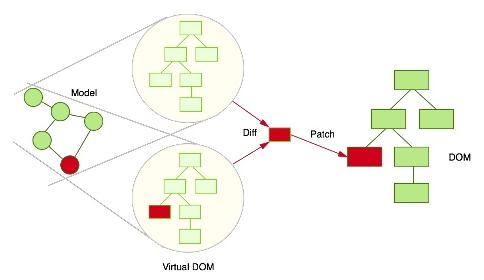
\includegraphics[scale=0.5]{./resources/vdom.jpg}
    \end{itemize}
\end{frame}
% -------------------------------------------------------------------------------------------------------------------------------------------------------------------
\begin{frame}{Jednosmeran tok podataka}
    \begin{itemize}
    	\item Nema vezivanja podataka
    	\item Komponenta zavisi samo od prosledjenih podataka
    	\item Stanje interfejsa je predvidivo i lako ponovljivo
    \end{itemize}
\end{frame}

% -------------------------------------------------------------------------------------------------------------------------------------------------------------------
\begin{frame}[fragile]{Redux}
    \begin{itemize}
    	\item Kontejner koji čuva stanje aplikacije
    	\item Osnovni princip
    	\begin{verbatim}
(prevState, action) => newState
    	\end{verbatim}
    \end{itemize}
\end{frame}

% -------------------------------------------------------------------------------------------------------------------------------------------------------------------
\begin{frame}{Tok upravljanja}
      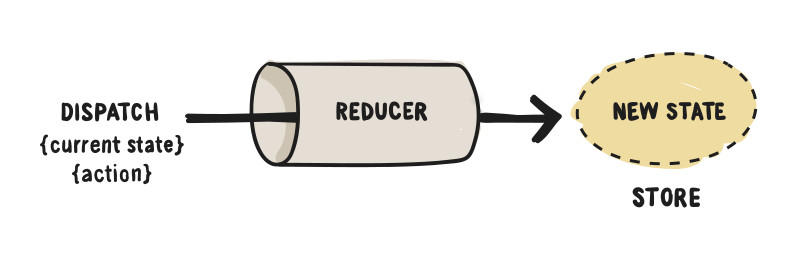
\includegraphics[scale=0.5]{./resources/redux.jpg}
\end{frame}

% -------------------------------------------------------------------------------------------------------------------------------------------------------------------

\end{document}
